\documentclass[10pt,a4paper]{article}
\usepackage[utf8]{inputenc}
\usepackage[english]{babel}
\usepackage{amsmath}
\usepackage{amsfonts}
\usepackage{amssymb}
\usepackage{graphicx}
\usepackage[left=3.5cm,right=3.5cm,top=3cm,bottom=3cm]{geometry}
\author{Fabian Schubert}
\title{Driven Random Dynamic Reservoir with Homeostatic Variance Control}

\parskip=5pt

\begin{document}
\begin{center}
\begin{LARGE}
\textbf{Driven Random Dynamic Reservoir with Homeostatic Variance Control}\\
\end{LARGE}
\end{center}

\section{Model Description}

\subsection{Dynamics}
\begin{align}
x_i^{t+1} &= \mathrm{tanh}\left( g_i^t I_i^{t+1} \right) \\
I_i^{t+1} &= \sum_{j=1}^{N_{\rm net}} W_{ij} x_j^t + \sum_{k=1}^{N_{\rm in}} E_{ik} e_k^{t+1} \\
g_i^{t+1} &= \mu_{g} \left[ \mathrm{Var_{target}} - \left( x_i^t - \langle x_i \rangle \right)^2 \right]
\end{align}

\subsection{Parameters / Settings}

$W_{ij}$ is a sparse random matrix with connection probability ${\rm cf_{net}}$. Nonzero entries were drawn from a Gaussian distribution $\mathcal{N}(\mu = 0,\sigma = \sigma_{\rm conn} / \sqrt{N_{\rm net} {\rm cf_{net}}})$. Diagonal entries were always set to zero.

$E_{ij}$ is also a sparse random matrix with connection probability ${\rm cf_{in}}$. Nonzero entries were drawn from a Gaussian distribution $\mathcal{N}(\mu = 0,\sigma = \sigma_{\rm conn} / \sqrt{N_{\rm in} {\rm cf_{in}}})$.

$e_i^{t}$ are activities of an input layer of size $N_{\rm in}$, which are independently drawn from a uniform $\rm \left[0,1\right]$ distribution for each time step. External input is turned off after $t_{\rm ext.off}$.

By changing individual gain values $g_i$, the homeostatic control tries to drive the activity variance of every cell to the value given by $\mathrm{Var_{target}}$. However, this mechanism is also switched off after $t_{\rm ext.off}$. This is done because we can assume that homeostatic processes would biologically act on much slower timescales than changes in input. Before $t_{\rm ext.off}$, we can set $\mu_{g}$ to relatively high values to let homeostasis converge under external drive.

See all parameters in Table \ref{tab:params}.
\begin{table}[h]
\caption{Model Parameters}
\centering
\vspace{5pt}
\begin{tabular}{l | r}
\textbf{Parameter} & \textbf{Value} \\
\hline
$N_{\rm net}$           & 500\\
$N_{\rm in}$            & 10\\
${\rm cf_{net}}$        & 0.1\\
${\rm cf_{in}}$         & 0.1\\
$\sigma_{\rm conn}$     & 1.0\\
$\mu_{g}$               & 0.0005\\
$\mathrm{Var_{target}}$ & 0.1\\
$n_t$ (Sim. Steps)      & 200000\\
$t_{\rm ext.off}$       & 100000
\end{tabular}
\label{tab:params}
\end{table}
\newpage
\section{Results}
Exemplary results are shown in Fig. \ref{fig:ex_results}.

\begin{figure}[h]
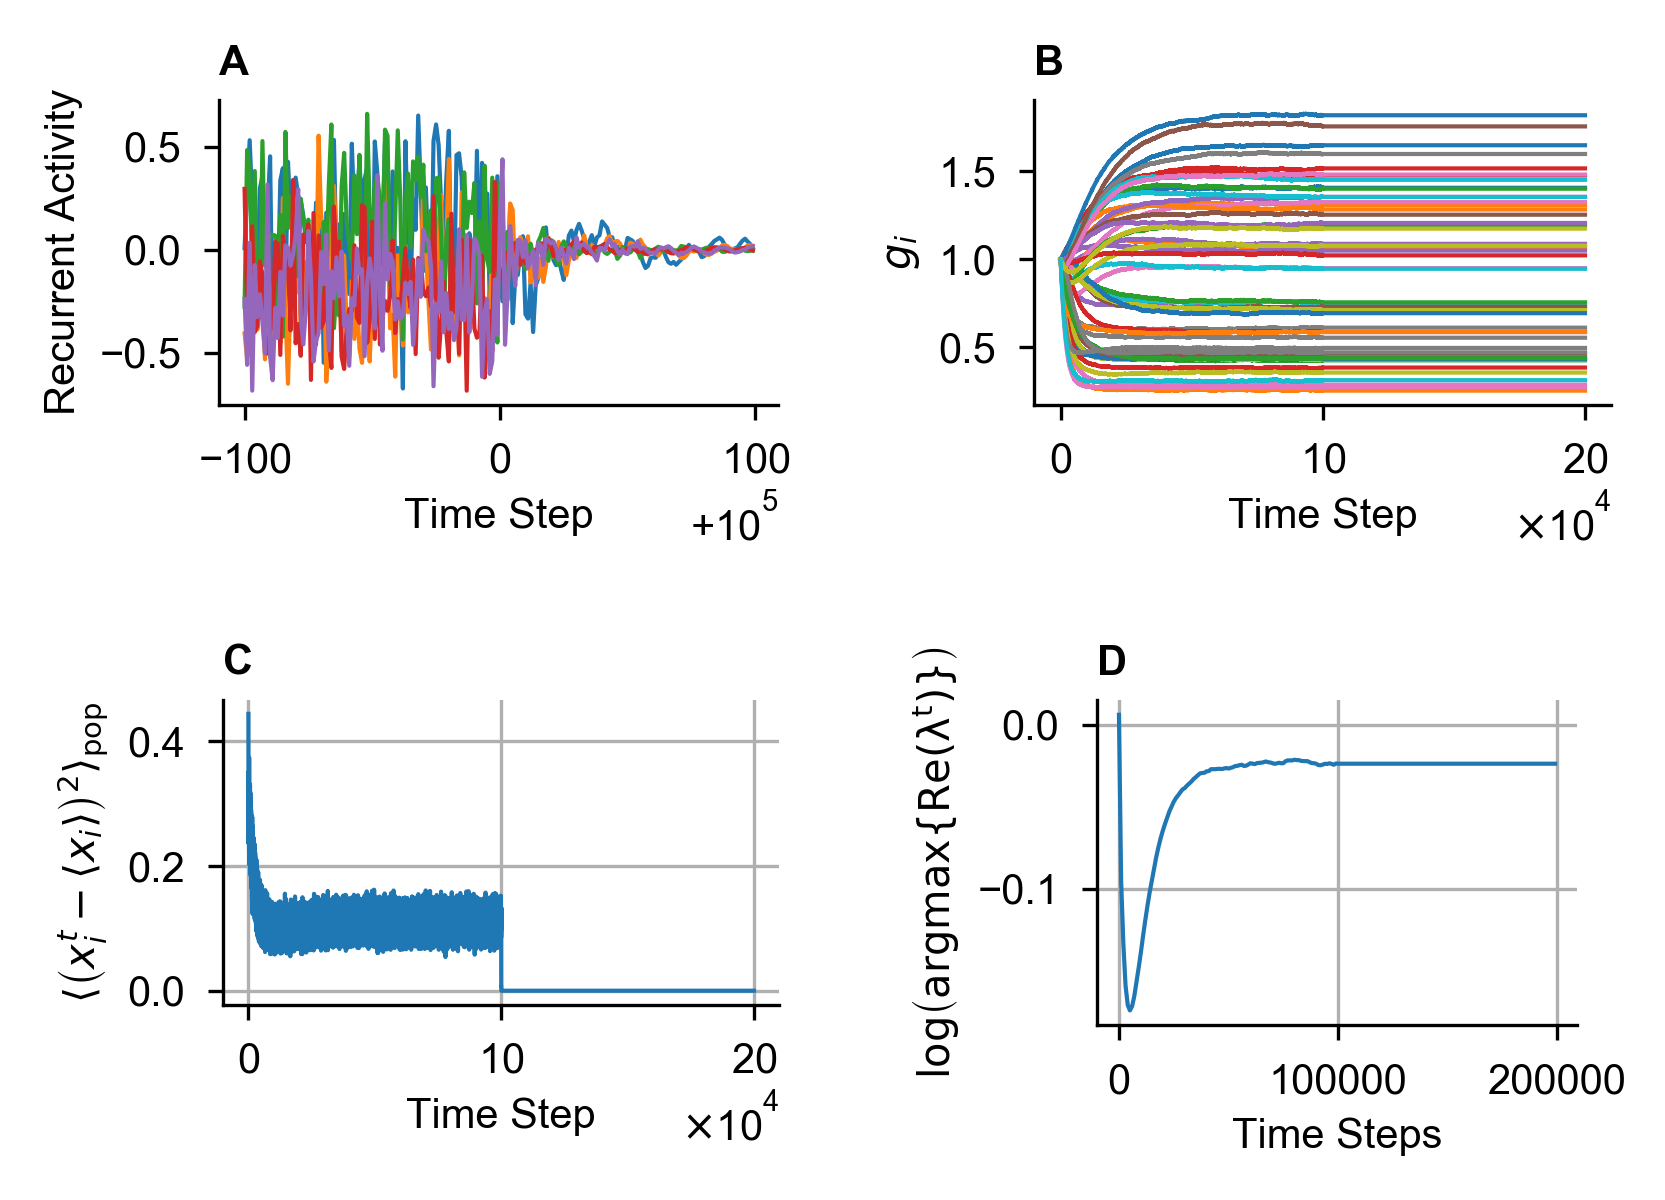
\includegraphics[width=\textwidth]{../plots/im_comp.png}
\caption{{\bf A}: Sample of activity within $\left[ t_{\rm ext.off} - 100, t_{\rm ext.off} + 100 \right]$. {\bf B}: Gain dynamics of $N_{\rm net}/10$ exemplary neurons. {\bf C}: Population mean of squared activity. {\bf D}: Log. of largest real part of eigenvalues of $g_i^t W_{ij} $.{\bf E}: Sample of population activity for the last 100 steps.}
\label{fig:ex_results}
\end{figure}


\end{document}